\chapter{Mapping}
\index{Mapping|(}
Tellervo includes an integrated open source 3D mapping system (based on NASA's award winning World Wind Java SDK) similar to the program Google Earth which you're no doubt familiar with. As mentioned in the installation chapter, this mapping system requires an OpenGL 3D capable graphics card. Before you can use the mapping in Tellervo, you must also have something to map! See the chapter on Metadata (page \pageref{txt:metadata}) for information about adding coordinates to your system.

There are two ways to map data from your database. First of all, you can see a map of all the sites (i.e. TRiDaS objects) by going to \menutwo{Administration}{Site map}. This will give you a screen like this:

\begin{figure}[hbtp]
  \label{fig:map}
  \centering
  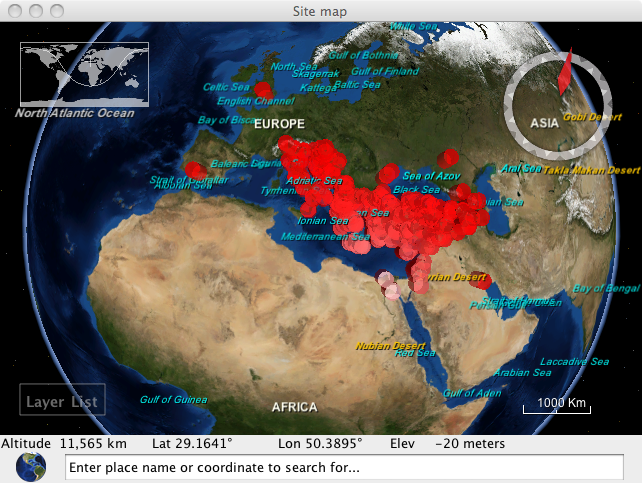
\includegraphics[width=\textwidth]{Images/sitemap.png}
  \caption{Screenshot showing an example of a site map.}
\end{figure}


You can also see a map of your current series if you have latitude/longitude metadata by clicking on the map tab on the main data screen.  
\newpage

\section{Navigation}
\index{Mapping!Navigation}
\begin{figure}[hbtp]
  \centering
  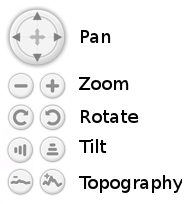
\includegraphics[width=0.2\textwidth]{Images/wwjcontrols.png}
  \caption{On-screen navigation controls.}
  \label{fig:wwjcontrols}
\end{figure}

You can navigate around your maps using the on screen controls (figure \ref{fig:wwjcontrols}), by using your mouse and/or your keyboard.  These controls enable you to explore your location information in 3D such as the example of Mount Vesuvius in figure \ref{fig:mappin}.




\subsection{Mouse with scroll wheel}

\begin{description*}
      \item[Pan] Left mouse button click and drag -- all directions
      \item[Zoom] Use the scroll wheel on the mouse or Left and Right mouse (both buttons) click and drag up and down
      \item[Tilt] Right mouse button click and drag -- up and down or use `Page Up' and `Page Down' on the keyboard.
      \item[Rotate] Right mouse button click and drag -- left and right Note: Crossing the top and bottom half of the screen while rotating will change direction.
      \item[Stop] Spacebar
      \item[Reset Heading] N
      \item[Reset all] R 
\end{description*}



\subsection{Single button mouse}
\begin{description*}
     \item[Pan] Left mouse button click and drag - all directions. L left mouse button click once to center view.
     \item[Zoom] Hold `Ctrl' on the keyboard and Left mouse button click and drag - up and down
     \item[Tilt] Hold `Shift' on the keyboard and Left mouse button click and drag - up and down or use "Page Up" and "Page Down" on the keyboard.
     \item[Rotate] Hold `Shift' on the keyboard and Left mouse button click and drag - left and right
     \item[Stop] Spacebar
     \item[Reset Heading] N
     \item[Reset all] R 
\end{description*}

%\begin{SCfigure}
%  \centering
%  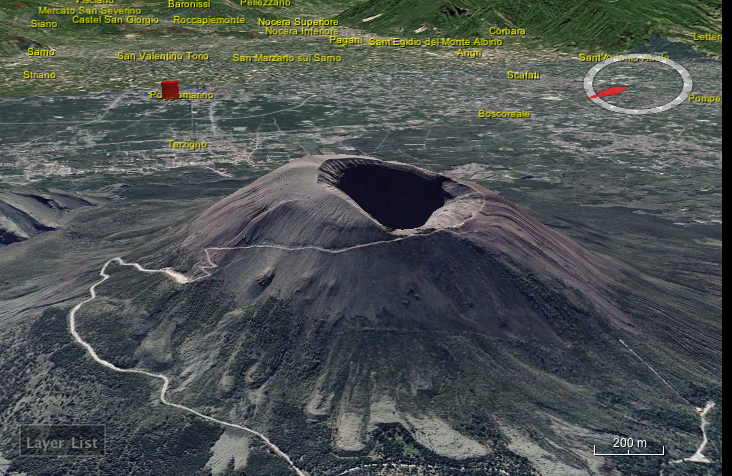
\includegraphics[width=0.8\textwidth]{Images/3dmapexample.png}
%  \caption{Example of 3D mapping in Tellervo.}
%  \label{fig:3dmap}
%\end{SCfigure}

Another method of navigating around the map is by using the built in gazetteer. You can enter and place name or coordinate information into the box at the bottom of the screen and you will fly to the requested location. 


\section{Interacting with data}

Each marker on the map represents either a TRiDaS object or element in your Tellervo database. By clicking on these pins you can get more information from the database (see figure \ref{fig:mappin}).

\begin{figure}[hbtp]
  \centering
  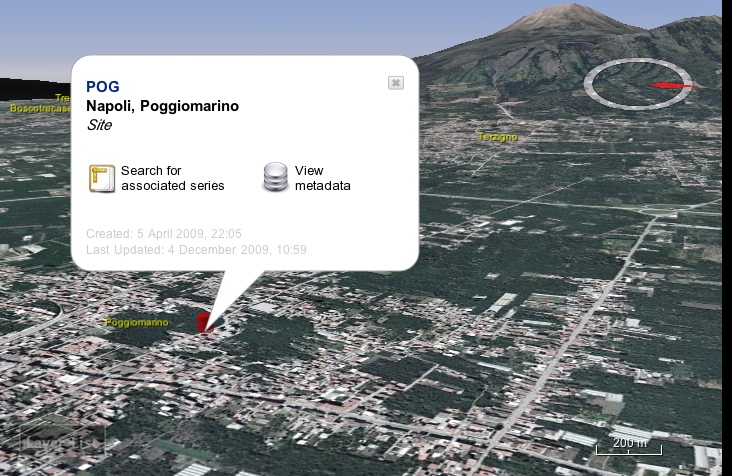
\includegraphics[width=0.8\textwidth]{Images/mappinexample.png}
  \caption{Screenshot of a map with information pin expanded}
  \label{fig:mappin}
\end{figure}

The example above shows the ring marker is of a site in Napoli called Poggiomarino (code name POG). You can see the option for searching for all series in the database associated with this site, and also the option for viewing all the metadata. 

\section{Map layers}
\label{txt:userAddWMS}
\index{Mapping!Layers}

Tellervo comes ready configured with basic map layers, including high resolution satellite imagery and basic political features. You can turn background layers on and off by going to \menutwo{View}{Layers} or using the layer panel at the left of the screen when using `Site map'.

Map layers are downloaded on-the-fly so there is likely to be a delay when you initially visit to a new region. However, up to 2Gb of map data can be cache locally to your hard disk, so on future visits, maps should load quickly.

\subsection{Data layers}
Data map layers (i.e.\ site and sample locations) are controlled with the layer list on the left of the screen. When viewing series, you will have the option of adding layers containing points for all the other series at the current site, and showing all the sites in the database. 

In the `Site map' you can use the `Add layer' button to add data layers of the following types:

\begin{description}
 \item[All Tellervo objects] -- this adds a single layer containing all the objects within the Tellervo database.
 \item[Tellervo entity from database] -- this adds a layer containing the location of one record from the Tellervo database.  This is specified by labcode e.g. ABC would add a pin for the site ABC, whereas ABC-1 would add a pin for the element ABC-1.
 \item[Elements from an object] -- this adds a layer containing all the elements for a specified object.  The object is specified by labcode.
 \item[All ITRDB sites] -- this downloads the location of all sites currently available in the ITRDB database and adds them as a single layer.
 \item[ESRI Shapefile] -- this enables you to load an ESRI shapefile stored locally on your computer.  Tellervo supports polygon, polyline and point files, although currently it does not enable you to style this data.  Data for a layer is presented using a random color.
 \item[Google Earth KML/KMZ file] -- like the ESRI shapefile option this enables you to load spatial data from your computer.
 \end{description}


\subsection{Web Map Service (WMS)}
\index{Web Map Service (WMS)}
\index{Mapping!Web Map Service (WMS)}

The mapping system in Tellervo includes support for remote map servers that use the OGC Web Mapping Service (WMS) standard. If you go to \menuthree{View}{Layers}{Add remote layers}, you will get a dialog with a tab for each WMS server configured for your system. By default this includes the NASA Earth Observation and Jet Propulsion Lab servers.  By ticking layers in this list you can add data layers to your map.

You can add map data from other WMS servers by clicking the `+' tab and entering the URL of the server you would like to use.  This will give an additional tab with all the available map layers.  This server will only be available for the duration of your current session so will need to be added each time you start Tellervo.  If you would like a particular WMS server to be made permanently available, your Tellervo administrator can do this (see `Managing map services', on page \pageref{txt:managingmaps} for further details).  Additional WMS servers added in this way will be available to all users the next time they connect to your Tellervo server.

Your system administrator may host a map server specifically for your lab, for instance, containing high resolution plans of an archaeological site that you are working on, or environmental data for your study region. Figure \ref{fig:wms} shows an example overlay of sea surfaces temperatures loaded dynamically from the NASA EO server.

\begin{figure}[hbtp]
  \centering
  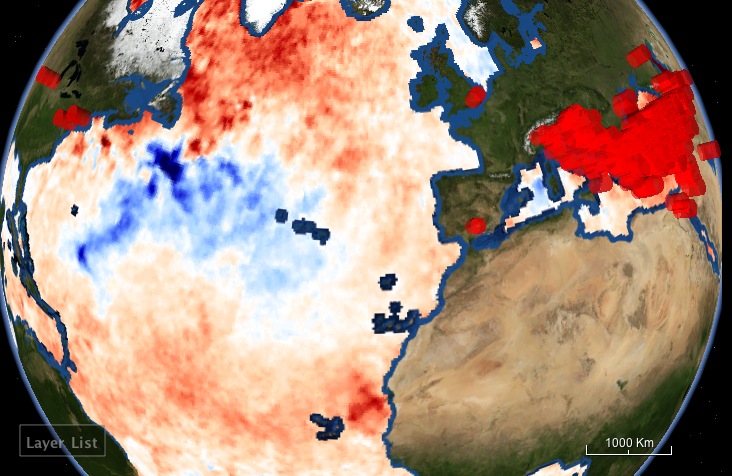
\includegraphics[width=0.8\textwidth]{Images/sst.png}
  \caption{Map screenshot with a NASA sea surface temperature overlay dynamically loaded from the NASA WMS server.}
  \label{fig:wms}
\end{figure}





\section{Exporting maps}
\index{Export!Maps}
You can export maps by going to \menutwo{File}{Export map as image}. For best results, maximize your map window first. You may also like to turn off various map widgets by going to the View menu. The exported image will include everything you can see on your map screen. 


\index{Mapping|)}